\documentclass[tikz,border=3mm]{standalone}
% общий стиль (подключается через TEXINPUTS)
% tikz-style.tex (общий стиль для всех TikZ-картинок)
\RequirePackage[T1,T2A]{fontenc}
\RequirePackage[utf8]{inputenc}

% Palatino-подобный шрифт (как в MathJax часто воспринимается «более вытянутым»)
\RequirePackage{txfonts}
% txfonts даёт предупреждение по кириллице (T2A/txr не определён).
% Оставляем txfonts для математики, а текстовый шрифт возвращаем на Computer Modern,
% чтобы не искать T2A/txr и убрать предупреждения.
\renewcommand{\rmdefault}{cmr}
\renewcommand{\sfdefault}{cmss}
\renewcommand{\ttdefault}{cmtt}

\RequirePackage{tikz}
\RequirePackage{xcolor}
\usetikzlibrary{calc}

% цвета
\definecolor{lightgreen}{RGB}{214,234,214}
\definecolor{darkgreen}{HTML}{0B7A0B}
\definecolor{darkred}{HTML}{DF0000}

\definecolor{midgreen}{HTML}{2E9B2E}
\definecolor{palegreen}{RGB}{235,246,235}
\definecolor{olivegreen}{HTML}{3E6B2F}

\definecolor{lightred}{RGB}{255,220,220}
\definecolor{midred}{HTML}{E04545}
\definecolor{darkred2}{HTML}{A80000}

\definecolor{lightblue}{RGB}{220,232,255}
\definecolor{midblue}{HTML}{2E5BD6}
\definecolor{darkblue}{HTML}{0B2E8A}

\definecolor{lightgray}{RGB}{240,240,240}
\definecolor{midgray}{RGB}{170,170,170}
\definecolor{darkgray}{RGB}{80,80,80}

\definecolor{vtxfill}{RGB}{86,193,255}
\definecolor{vennfill}{RGB}{220,232,255}


% единый набор стилей TikZ
\tikzset{
    lab/.style={
        font=\fontsize{24}{32}\selectfont
    }
}

\usetikzlibrary{matrix,positioning}

\begin{document}
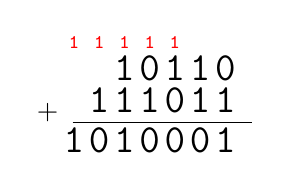
\begin{tikzpicture}[font=\rmfamily\Large]
\matrix (m) [
matrix of nodes,
column sep=0.6mm,
row sep=0.8mm,
nodes={anchor=base, inner sep=0pt},
column 1/.style={nodes={anchor=east, font=\rmfamily}},
anchor=west
] {
 & {\scriptsize\textcolor{red}{\ttfamily 1}} & {\scriptsize\textcolor{red}{\ttfamily 1}} & {\scriptsize\textcolor{red}{\ttfamily 1}} & {\scriptsize\textcolor{red}{\ttfamily 1}} & {\scriptsize\textcolor{red}{\ttfamily 1}} & {} & {} \\
 & {} & {} & {\ttfamily 1} & {\ttfamily 0} & {\ttfamily 1} & {\ttfamily 1} & {\ttfamily 0} \\
{\rmfamily +} & {} & {\ttfamily 1} & {\ttfamily 1} & {\ttfamily 1} & {\ttfamily 0} & {\ttfamily 1} & {\ttfamily 1} \\
 & {\ttfamily 1} & {\ttfamily 0} & {\ttfamily 1} & {\ttfamily 0} & {\ttfamily 0} & {\ttfamily 0} & {\ttfamily 1} \\
};

\draw ([xshift=-2mm,yshift=-0.8ex]m-3-3.west |- m-3-3.south)
  -- ([xshift=2mm,yshift=-0.8ex]m-3-8.east |- m-3-3.south);

\end{tikzpicture}
\end{document}
